\documentclass[letterpaper,11pt]{article}
\usepackage[parfill]{parskip} % Remove paragraph indentation
\usepackage{amsmath}
\usepackage{float}
\usepackage[margin=1in]{geometry}
\usepackage{graphicx}
\usepackage{placeins}
\usepackage{siunitx}
\usepackage[title]{appendix}
\usepackage{pdflscape}
\usepackage{tabularx}
\usepackage{times}
\usepackage{url}
\usepackage{setspace}
\usepackage[none]{hyphenat}
\usepackage{pdfpages}
\usepackage{longtable}
\usepackage{tikz}
\usepackage{hyperref}
\usepackage{minted}

\DeclareSIUnit{\samplepersec}{SPS}
\newcommand{\code}[1]{\mintinline{systemverilog}{#1}}

\begin{document}

\begin{titlepage}
    \begin{center}
        \vspace*{1cm}

        \Large
        \textbf{ELEC 490/498 Project Final Report}

        \vspace{0.5cm}
        Group 18\\
        TeachEE: Accessible Electronics Instrumentation\\
        \vspace{0.5cm}
        \normalsize
        \textbf{John Giorshev (20103586, john.giorshev@queensu.ca) \\ Eric Yang (20120750, e.yang@queensu.ca) \\ Ethan Peterson (20105011, 17emp5@queensu.ca) \\ Timothy Morland (20096286, 17tm22@queensu.ca)}\\
        \vspace{0.5cm}
        Submitted April 10, 2023\\

        \vfill
            
        \textbf{To:}\\
        Instructor Dr. Michael Korenberg (korenber@queensu.ca) \\
        Instructor Dr. Alireza Bakhshai (alireza.bakhshai@queensu.ca) \\
        Instructor Dr. Alex Tait (alex.tait@queensu.ca) \\
        Instructor and Supervisor Dr. Sean Whitehall (sw109@queensu.ca) \\
        Supervisor Dr. Thomas Dean (tom.dean@queensu.ca) \\
            
        \vspace{1.8cm}

    \end{center}
\end{titlepage}
\setstretch{1.5}
\pagenumbering{gobble}
\section*{Executive Summary}
% ERIC OWNS THIS SECTION
EXEC SUMMARY HERE

\newpage

\setstretch{1}
\tableofcontents
\listoffigures
\listoftables
\newpage
% upgraded this to double spacing as per report formatting reqs
\setstretch{2}
\pagenumbering{arabic}
\section{Motivation \& Background}
% ERIC
% Motivation and background – a clear problem statement and the motivation for the
% project (why is it technologically interesting?). A good motivation argument
% usually relies on facts and figures about the technological void that you seek
% to fill with your design. Back-up your facts and figures by referencing archival
% references. Examples of archival references include: journal papers, conference
% papers, patents, books, corporate technical and annual reports, application
% notes. Use the standard IEEE citation format. Website URLs are not archival
During the Covid-19 pandemic, many universities abruptly switched to remote
learning as campuses were shut down. This sudden change exposed the lack of
support for more digital learning models \cite{online_learning}. Although the
pandemic has since passed, forward-thinking institutions are starting to invest
in online programs, for example, by leveraging AI chatbots and teaching assistants.
Additionally, online course providers such as Udemy have recently risen in popularity
as a cheap alternative to traditional postsecondary education. With this trend of
remote higher education, engineering students will need their own lab equipment to
complete their learning requirements.

TeachEE is a user friendly general purpose electronics measurement instrument
designed for remotely delivered engineering labs. It acts as both a
USB oscilloscope and current monitor. Currently, there are few instrumentation
options for students completing their labs remotely. The oscilloscopes used for
onsite learning are bulky and difficult to use. TeachEE bundles
together the functionality most commonly required for electrical engineering
labs and packages it with portable software that can run on lower end computers
with any operating system.

\section{Design}
%% Design – describe your functional requirements and constraints; provide
%% technical details about your design process for meeting the project goals;
%% this might include identifying subsystems, analysis, modeling, and key
%% decisions made. If your project involves circuit design, you should describe
%% the simulations used to create your design

% Summarize Design process of hardware, fpga and SW. Make a brief note about how
% we parallelized much of the work by modelling the data as a byte stream.
% allowing for significant dev work without physical HW in house.

The TeachEE design is derived from the system requirements set in the blueprint
report. Given in Table \ref{tab:hw-reqs} and \ref{tab:sw-reqs} are the hardware
and software requirements respectively. It should also be noted that the FPGA
shares responsibility with the desktop application for fulfilling software
requirements.

\begin{table}[H]
    \caption{Hardware Requirements}
    \begin{tabularx}{\textwidth}{l|l|l|l}
          & Specification & Target Value & Tolerance \\
        \hline
        1 &Voltage Input Bandwidth&\SI{100}{\kilo\hertz}& $\pm \SI{1}{\kilo\hertz}$ \\
        2 &Current Input Bandwidth&\SI{100}{\kilo\hertz}& $\pm \SI{1}{\kilo\hertz}$ \\
        3 &Measureable Current Range&\SI{-15}{\ampere} to \SI{+15}{\ampere}& $\pm \SI{5}{\ampere}$ \\
        4 &Measureable Voltage Range&\SI{0}{\volt} to \SI{3.3}{\volt}& $\pm \SI{200}{\milli\volt}$ \\
        5 &Number of Current Input Channels& $1$ & $0$ \\ 
        6 &Number of Voltage Input Channels& $1$ & $+2$ \\
        7 &Power Input Voltage Rating& \SI{5}{\volt} & $\pm \SI{500}{\milli\volt}$ \\
        8 &Power Current Consumption Rating& \SI{500}{\milli\ampere} & $\pm \SI{250}{\milli\ampere}$ \\
        9 &Voltage Sample Rate& \SI{1}{\mega\samplepersec} & \SI{0}{\mega\samplepersec}\\
        10 &Current Sample Rate& \SI{1}{\mega\samplepersec} & \SI{0}{\mega\samplepersec} \\
        11 &PCB Thickness& \SI{1.6}{\milli\metre} & $\pm \SI{0.1}{\milli\metre}$ \\
        12 &PCB Dimensions& \SI{0.04}{\meter\squared} & $\pm \SI{400}{\milli\metre\squared}$ \\
        13 &Voltage Sample Error against commercial scope & N/A & $\pm \SI{20}{\percent}$ \\
        14 &Current Sample Error against commercial meter& N/A & $\pm \SI{20}{\percent}$
    \end{tabularx} 
\label{tab:hw-reqs}
\end{table}

\begin{table}[H]
  \caption{Software Requirements}
  \begin{tabularx}{\textwidth}{l|l}
    \textbf{1} & \textbf{Functional Requirements}\\
    \hline
    1.1 & The software shall be able to modify the horizontal and vertical scales of the plot. \\
    1.2 & The software shall be able to modify the trigger voltage. \\
    1.3 & The application shall be deployable to Windows, macOS, and Linux. \\
    \hline
    \textbf{2} & \textbf{Interface Requirements} \\
    \hline
    2.1 & The software shall be able to capture voltage samples and export them to a CSV file. \\
    2.2 & The software shall receive samples via the FTDI 232 in synchronous mode. \\
    \hline
    \textbf{3} & \textbf{Performance Requirements} \\
    \hline
    3.1 & The software shall be able to render waveforms at a rate of \SI{30}{\hertz} on screen.
  \end{tabularx} 
  \label{tab:sw-reqs}
\end{table}

Based on the system requirements, the project is broken up into three
subsystems; hardware, FPGA, and software. The following subsections correspond
to each subsystem. Each section describes the subsystem's top level design, and
key design decisions made to comply with system requirements.

% INCLUDE THE BLOCK DIAGRAMS FOR EACH OF THESE
% Talk about old design (from blueprint)
\subsection{Hardware} % Ethan
The primary design driving requirements for the Printed Circuit Board (PCB) are
the bandwidth and sample rate of the data acquisition channels. Bandwidth and
sample rate constrain the selection of the input filters and Analog to Digital
Converters (ADCs) on the PCB. After selecting these parts, they can be easily
duplicated to add additional channels. The power requirements for the hardware
are trivial in comparison as they are already in alignment with the power
interface supplied by a standard USB port. The physical dimension requirements
of the PCB are also comparatively simple as the parts are easily packed more
closely using modern PCB layout and assembly techniques. A full requirement
compliance check for the hardware and other subsystems is provided in Section
\ref{sec:testing}.

Given the requirement for a single voltage and current channel with room for
additional voltage channels, the team settled on a four-channel design. One ADC
channel would be used for current and another for voltage. The remaining two
channels would be made available to the on-board FPGA should the team have the
time to add additional channels. The two spare channels would also have a higher
sample rate to improve the utility of the instrument.

It should be noted that all the data acquisition channels are connected to an
FPGA rather than a microprocessor. This decision was made to ensure we had no
real time data processing limitations and precise timing in our sampling of the
signal waveforms. Moreover, it is common with existing commercial oscilloscopes
to have an FPGA or ASIC fulfill these real time requirements. One compromise
that was made in the design was the use of an FPGA module rather than installing
the chip to the PCB directly. While such a module could not be used in TeachEE
in a mass-production setting, it greatly shortened the PCB design time, and
allows the FPGA to be easily replaced in the event of hardware failure.
Moreover, the FPGA combines all the sample streams and provides a single point
of contact to the USB interface.

Figure \ref{fig:hw-block-diagram} is a complete hardware block diagram used as a
guide for the PCB design implementation.

\begin{figure}[h]
  \centering
  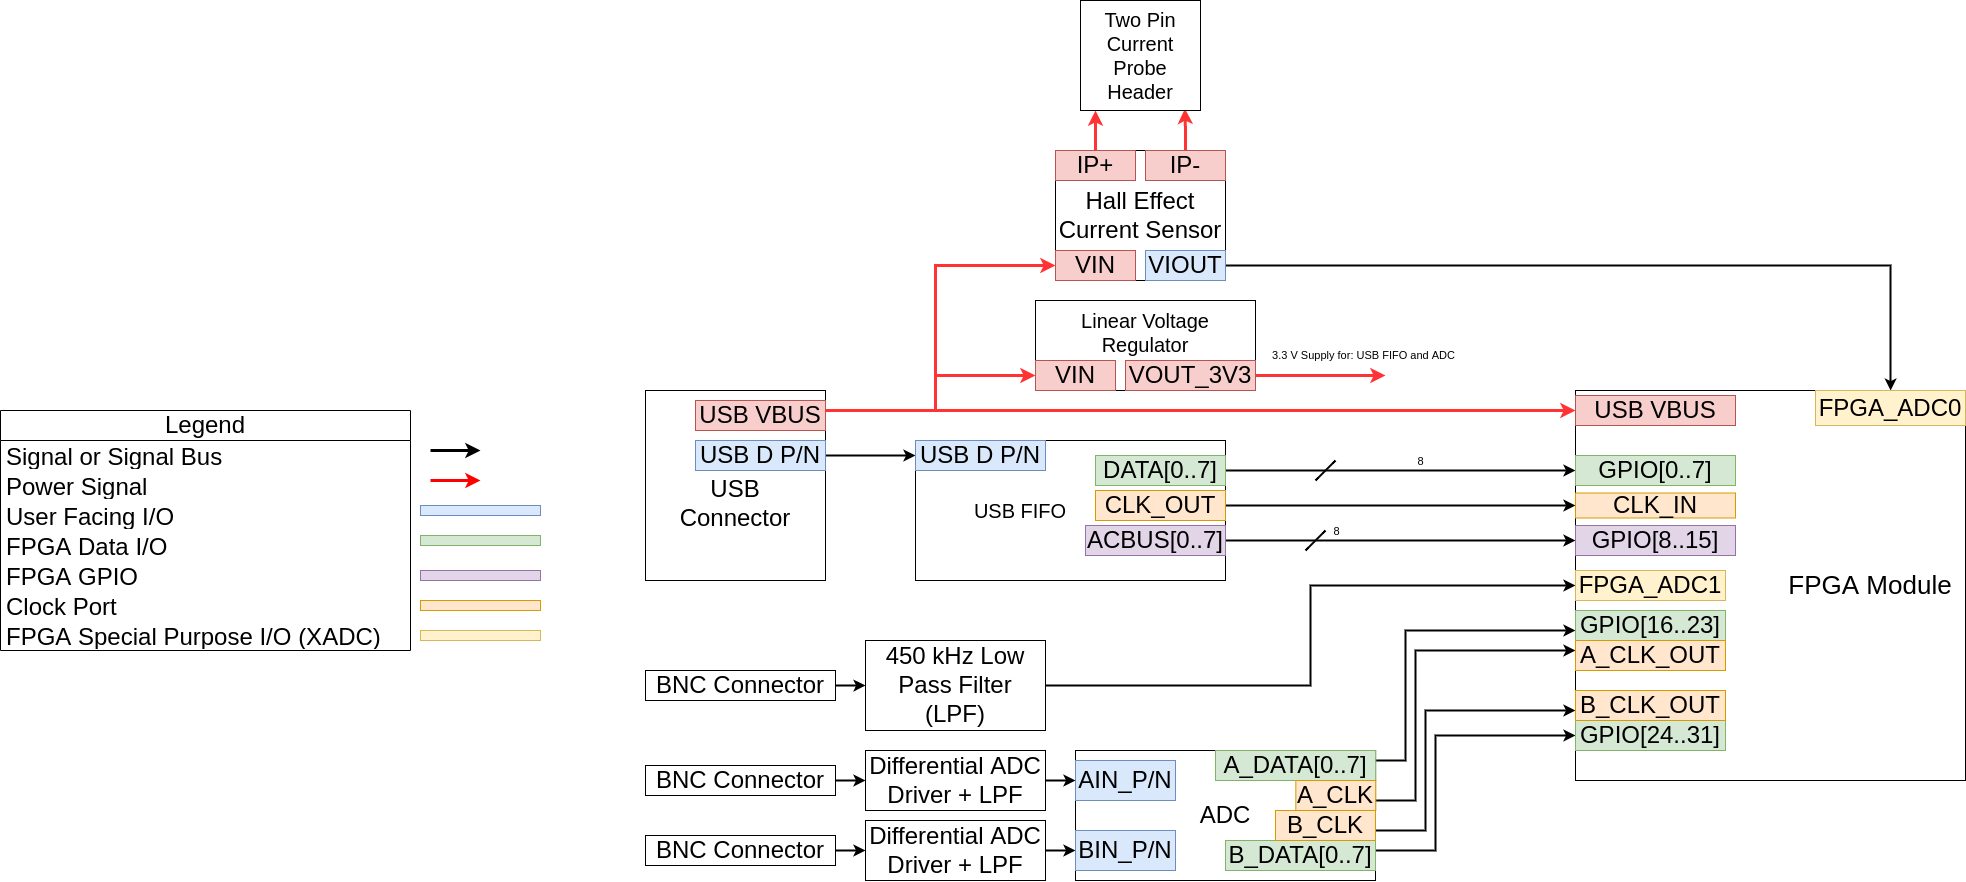
\includegraphics[width=\textwidth]{../../misc/TeachEE-System-Diagram-Hardware.png}
  \caption{Hardware System Block Diagram}
  \label{fig:hw-block-diagram}
\end{figure}

\subsection{FPGA} % Ethan
The FPGA RTL is primarily driven by the implicit requirement to send multiple
streams of data with low latency. The sample rate and bandwidth requirements are
not as concerning in the design of the FPGA subsystem. This is because sample
rates can be easily tuned in the FPGA with clock generation PLLs and bandwidth
depends on the analog bandwidth of the input circuitry on the PCB.

In order to transmit multiple streams, the FPGA needs to frame multi-channel
data in a standard packet format. A multiplexer is also used for a case where
sending all data at once is too much throughput for USB 2.0. With these issues
in mind, the diagram given in Figure \ref{fig:fpga-block-diagram} provides a
system-level block diagram for the FPGA design.

\begin{figure}[h]
  \centering
  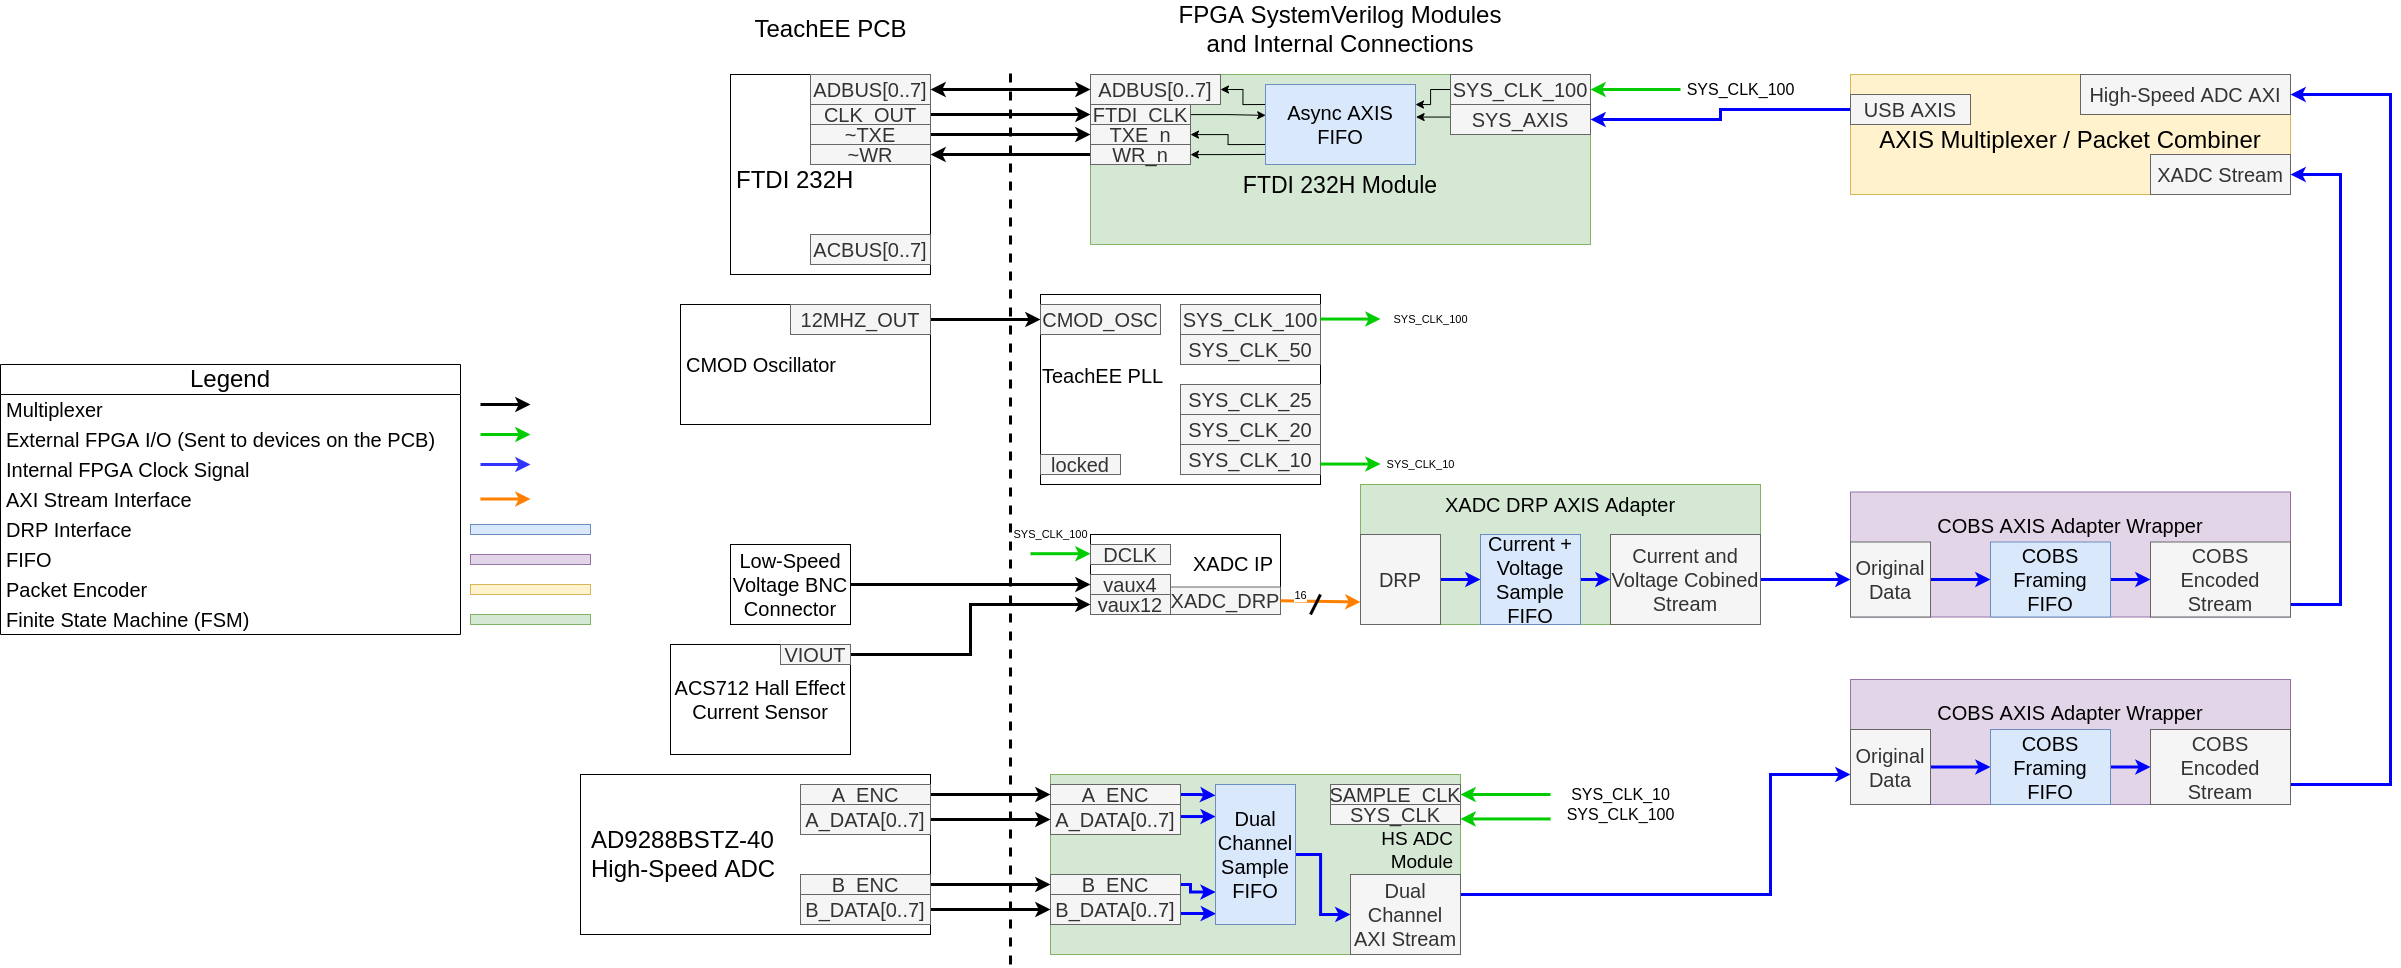
\includegraphics[width=\textwidth]{../../misc/TeachEE-System-Diagram-FPGA.png}
  \caption{FPGA System Block Diagram}
  \label{fig:fpga-block-diagram}
\end{figure}

A full breakdown of Figure \ref{fig:fpga-block-diagram} is given in the Section
\ref{sec:impl} focusing on implementation. Overall, the initial design is nearly
identical to the final implementation. The team made use of COBs packet encoding
as promised in the blueprint and added a standard AXI Streaming protocol for the
internal FPGA datapath.

\subsection{Software} % Tim
% Tauri, two threaded one buffer guarded with mutex

\section{Implementation} \label{sec:impl}
%% Describe how the solution was implemented – this may involve a description of
%% major code blocks, schematics, photographs, CAD drawings, etc. The reader
%% should understand the materials and operation of your implemented project,
%% and the tools (hardware and/or software) used. This should also include a
%% full bill of materials and final project budget.

% Discuss how everything was implemented here
% Ethan will include figure of top level altium schematic
% Ethan will also include snippet of the top level SystemVerilog Module.
% I will pull in full schematics, layout and code into the appendices

The implementation is broken up into three subsections corresponding to each
subsystem.

\subsection{Hardware} % ETHAN
The hardware solution for the TeachEE is implemented in the form of a four-layer
PCB. The PCB is designed using the EDA CAD software Altium Designer. Altium is
the industry standard tool for PCB design. Our design takes advantage of
Altium's hierarchical schematics. This allows the schematic to be broken up into
multiple pages with interconnects between the different sub-circuits. The
TeachEE's top level schematic is an interconnect between all the sub-circuits of
the PCB. The top level schematic is shown in Figure
\ref{fig:hw-top-level-sheet}. It should be noted that all 8 pages of the
schematic are provided in Appendix \ref{appendix:schematic}.

\begin{figure}[h]
  \centering
  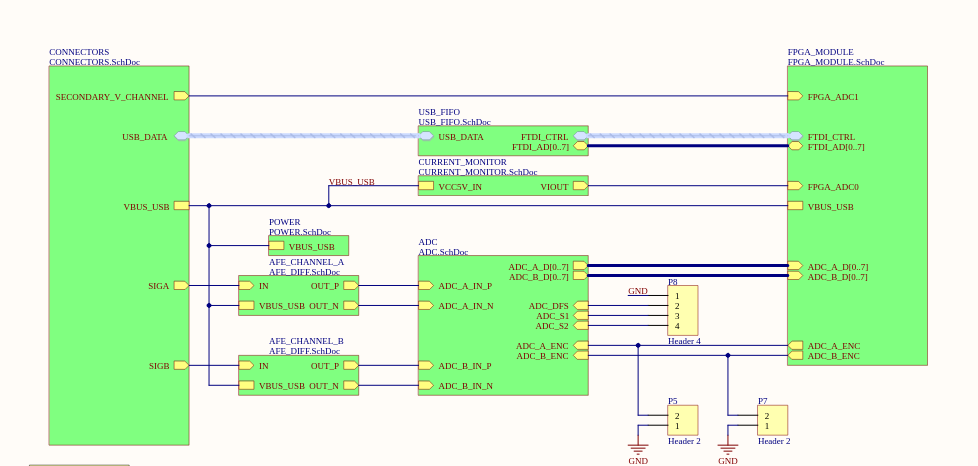
\includegraphics[width=\textwidth]{figures/altium-top-level.png}
  \caption{TeachEE PCB Top Level Schematic}
  \label{fig:hw-top-level-sheet}
\end{figure}

The following subsections break down each sub-circuit sheet entry in Figure
\ref{fig:hw-top-level-sheet}.

\subsubsection{Power}
The power schematic sheet contains a single LD1117V33C linear voltage regulator.
The regulator takes the 5V VBUS supply from the USB connection and provides a
3.3V power output. A linear voltage regulator is employed over a switching buck
converter for the following reasons.
  \begin{enumerate}
    \item The analog to digital converters require clean voltage references to
      produce accurate readings and function correctly. Buck converters are
      typically have more noisy outputs that could harm performance.
    \item The linear voltage regulator requires less components to implement
      easing chip shortage concerns.
    \item The significantly lower efficiency of a linear regulator is not an
      issue as this regulator has a capacity of 1A which is more than enough to
      run the devices on-board.
  \end{enumerate}
\subsubsection{USB FIFO}
The USB FIFO is a queue that sends data out to the laptop over USB 2.0 Full
Speed (FS). USB 2.0 FS is capable of up to 480 Mpbs. This circuit takes a
parallel byte stream from the FPGA and converts it to a USB 2.0 data stream. The
FT232HQ USB FIFO made by FTDI is used to implement this functionality. This chip
was selected over other USB Interface ICs for the following reasons.
  \begin{enumerate}
    \item Availability. USB Interfaces are one of many ICs in short supply
      in the ongoing chip shortage. In fact, this IC was ordered for the
      project after ELEC390 in July 2021 and only received in August 2022.
    \item Extensive pre-existing software tooling. FTDI provides a driver and
      configuration utility for extracting data from their USB interfaces. This
      significantly reduces the software development work required to build a
      sample streaming interface. This ease of use is critical in a project with
      such a short timeline.
  \end{enumerate}

For debugging and circuit visibility, all digital control signals on the
FT232HQ are connected to testpoints. The schematic sheet also contains some
surrounding circuitry in the form of power filtering, a clock oscillator, and
configuration EEPROM.

\subsubsection{Current Monitor}
The current monitor page contains a hall effect current sensor circuit. The
circuit makes use of the ACS720KLATR current sensor. This sensor was chosen due
to its supply chain availability and the fact that it reports its reading
through a voltage output. The voltage output is linearly proportional to the
current flowing through the sensor plus a DC offset. This is a preferred
interface as it can be simply connected to a ADC channel without having to write
a whole new driver for the specific sensor on the FPGA. As such, the output of
the current sensor is connected FPGA\_ADC0, which is one of two ADC channels
available on the FPGA module.

\subsubsection{ADC}
The TeachEE ADC schematic sheet contains AD9288BSTZ dual channel 40MSPS ADC.
This chip provides two additional high-speed voltage channels on top of the ADC
channels provided directly on board the FPGA module. The data outputs for both
channels A and B are sent to the FPGA along with the sample clocks. This ADC was
selected for its FPGA friendly control interface. Since the control consists of
only a data bus and sample clock, it is trivial to write an FPGA module to
collect the data in comparison to other SPI and I2C based converters on the
market.

Bypass capacitors and ferrite beads are used to power the ADC for the cleanest
reference voltage possible. Additionally, the PCB contains non-populated
footprints for low pass filters, and filter bypasses to simplify testing and
debugging. For the digital side, all data bus and clocks have test points so a
multimeter or oscilloscope can be connected to debug the FPGA control signals.

\subsubsection{Analog Front End (AFE)}
The Analog Front End (AFE) sits in front of the inputs of the high-speed ADC. As
a result, the sub-circuit is duplicated twice in the top level sheet shown in Figure
\ref{fig:hw-top-level-sheet} to cover both channels. The AFE serves the following
purposes in the data acquisition hardware.

\begin{enumerate}
  \item Protect the ADC from over-voltage conditions. The front-end must clamp
    any voltages that would otherwise destroy the ADC.
  \item Convert the signal from single ended to differential. The ADC takes in a
    differential input, so the AFE must convert the input voltage observed at
    the connector to a differential signal of equivalent magnitude.
\end{enumerate}

This functionality is implemented in hardware using an AD8138 differential ADC
driver. This ``all-in-one'' component takes care of voltage clamping and
single to differential conversion. Moreover, it has sufficient analog bandwidth
to avoid reducing the effective bandwidth of the ADC. For debugging, the
sub-circuit contains 0-ohm bypass resistors that can be optionally soldered to
send the unclamped signal directly to the ADC.

\subsubsection{FPGA Module}
The FPGA module is implemented using a CMOD A7-35T Xilinx Spartan 7 Breakout
Board. the module is connected to the PCB via two 28-pin headers. Two pins are
used for power and ground while the rest are used for FPGA IO pins. The USB FIFO
and ADC control pins are connected to the FPGA IO. There also two special IO,
which can be used as ADCs. These two pins are used to implement the current and
voltage channels at 1MSPS. The current sensor output is wired to one of the
channels and a BNC connector is connected to the other through a low pass filter
for voltage sampling.

The FPGA module schematic had one mistake that was not discovered until the
physical PCBs had already been manufactured and delivered. In order to use the
parallel-bus interface of the FT232HQ to send data, the FPGA must lock to a 60
MHz output clock from the FT232HQ. During the layout, the FPGA pin wired to this
clock was swapped to a normal GPIO pin rather than an MRCC dedicated clock pin.
As a result, the FPGA place and route was failing during compilation as the FPGA
could not route this clock from a standard GPIO pin. This issue was resolved by
waiving the warnings and optimizing the SystemVerilog code to still pass timing
without a proper clock route for the 60 MHz signal. Further information on this
process is given in Section \ref{sec:fpga-impl} on the FPGA implementation.

\subsubsection{Connectors}
% Talk about LPFs and BNC connectors 
The connectors page contains all the external IO connections for TeachEE.
Specifically, the USB mini connector for data and three BNC connectors for scope
probes. The current sensor is exposed on its own separate pin header. The BNC
connectors are connected to the appropriate ADC input or AFE. Also, each
connectors has the appropriate low pass filters to satisfy nyquist theorem. Each
connector also includes all the standard capacitors and resistors needed to
connect an oscilloscope probe from the lab kit sold at the Queen's bookstore.
\subsection{FPGA} \label{sec:fpga-impl} % ETHAN
% Refer to system block diagram and go module by module.
% put in the top level module code and some critical state machines
% Talk about AXIS as a standard protocol. Also the extensible to ARM SOCs it
% provides

The FPGA datapath and implementation can be best summarized by examining the
interconnections between modules in the top-level SystemVerilog module. Below is
each section of the top level TeachEE RTL module broken down and explained. The
entire RTL codebase can be viewed in Appendix \ref{appendix:rtl-code}.

\subsubsection{Top Level Module Interface}
Given below is the interface to the top level module of the TeachEE RTL code.

\setstretch{1}
\begin{minted}{systemverilog}
module teachee (
  input  var logic cmod_osc, // 12 MHz provided on the CMOD
  input  var logic ftdi_clk, // 60 MHz provided by the FTDI

  // FTDI Control Interface
  input  var logic ftdi_rxf_n,
  input  var logic ftdi_txe_n,

  output var logic ftdi_rd_n,
  output var logic ftdi_wr_n,
  output var logic ftdi_siwu_n,
  output var logic ftdi_oe_n,

  output var logic[7:0] ftdi_data,

  // High Speed ADC IO Interface
  output var logic hsadc_a_enc,
  input var logic[7:0] hsadc_a,

  output var logic hsadc_b_enc,
  input var logic[7:0] hsadc_b,

  // CMOD IO Declarations
  input var logic[1:0] btn,
  output var logic[1:0] led,

  input var logic[1:0] xa_n,
  input var logic[1:0] xa_p,

  // TeachEE IO Declarations
  output var logic[1:0] teachee_led,
  inout wire[5:0] spare_pin
);
\end{minted}
\setstretch{2}

As shown above, the FPGA takes in one 12 MHz clock provided by an external
oscillator and the 60 MHz clock from the FT232HQ. After the clocks, IO for the
FT232HQ and AD9288BSTZ control signals are defined. At the end of the interface
declaration are pins for the FPGA module analog channels and some debug buttons
and LEDs on the TeachEE PCB.

\subsubsection{PLL Clock Generation}
After the module interface is declared, the PLL system clock generator is
initialized. This is an IP core provided by the FPGA manufacturer Xilinx that
takes the oscillator 12 MHz input and outputs a variety of useful clock signals
for the rest of the design. Given below is the IP core module instantiation.

\setstretch{1}
\begin{minted}{systemverilog}
    teachee_pll teachee_pll_ip_inst (
        // Clock out ports
        .clk_100(clk_100),     // output clk_100
        .clk_50(clk_50),     // output clk_50
        .clk_25(clk_25),     // output clk_25
        .clk_20(clk_20),     // output clk_20
        .clk_10(clk_10),     // output clk_10

        // Status and control signals
        .reset(0), // input reset
        .locked(locked),       // output locked

        // Clock in ports
        .cmod_osc(cmod_osc)      // input cmod_osc
    );
\end{minted}
\setstretch{2}

The module takes the external oscillator clock as an input and outputs 100, 50,
25, 20 and 10 MHz clocks. Different frequencies can be specified within the
Xilinx Vivado IDE used to flash the FPGA. In the current implementation, only
the 100 and 10 MHz clocks are used. 100 MHz is used throughout the top level
system and 10 MHz is used as a sampling clock in the high speed ADC. One clock
that is not covered by this PLL is the 60 MHz clock generated externally by the
FT232HQ. The PLL also has a \code{locked} output. When driven high, this signal
indicates that the PLL is locked to the input clock and the output clocks are
functioning correctly. This signal is used to create a reset signal to all the
modules holding them in reset until the PLL has locked and all clocks are up and
running.

\subsubsection{Interface Instantiations} \label{sec:interface-inst}

Given below are the instantiations for the different interfaces used to make
connections between the sub-modules. Interfaces in SystemVerilog can be thought
of as groupings of wires that make managing inter-module connections easier as
each wire does not need to be explicitly declared.

\setstretch{1}
\begin{minted}{systemverilog}
    hsadc_interface hsadc_ctrl ();
    assign hsadc_a_enc = hsadc_ctrl.channel_a_enc;
    assign hsadc_ctrl.channel_a = hsadc_a;

    assign hsadc_b_enc = hsadc_ctrl.channel_b_enc;
    assign hsadc_ctrl.channel_b = hsadc_b;

    assign hsadc_ctrl.s1 = spare_pin[0];
    assign hsadc_ctrl.s2 = spare_pin[1];
    assign hsadc_ctrl.dfs = spare_pin[4];

    axis_interface #(
        .DATA_WIDTH(2 * XADC_DRP_DATA_WIDTH)
    ) xadc_sample_channel (
        .clk(sys_clk),
        .rst(reset)
    );

    axis_interface #(
        .DATA_WIDTH(16)
    ) hsadc_sample_channel (
        .clk(sys_clk),
        .rst(reset)
    );

    axis_interface #(
        .DATA_WIDTH(8)
    ) hsadc_usb_axis (
        .clk(sys_clk),
        .rst(reset)
    );

    axis_interface #(
        .DATA_WIDTH(8)
    ) xadc_usb_axis (
        .clk(sys_clk),
        .rst(reset)
    );
\end{minted}
\setstretch{2}

The first interface declared is for the AD8138ARZ high-speed ADC. External IO
signals are assigned to the different control wires in the interface. Next, the
various AXIS interfaces required to connect the modules are instantiated. The
interface width is specified using the \code{DATA_WIDTH} parameter. 8-bit
interfaces are used to connect the packet stream output for a given ADC to the
FT232HQ wrapper module which adapts the AXI Stream to FT232HQ control signals.
The remaining two interfaces hold the sample data from the XADC and high-speed
ADC respectively. The XADC is the dual channel 16-bit ADC built into the FPGA.
The two sample data interfaces \code{hsadc_sample_channel} and
\code{xadc_sample_channel} are each connected to the outputs of adapter modules
that adapt the native interface of the device to an AXI Stream. The AXI Stream
interface used is a custom wrapper for all the standard signals found in an AXI
stream. The interface definition can be found in Appendix
\ref{appendix:axis-interface}.

The AXIS Protocol, also known as AXI Stream is derived from ARM's AXI bus
specification. Additional information on the AXI Stream protocol and the
external libraries used to support it can be found in Section
\ref{sec:external-fpga-libs}.

\subsubsection{FT232HQ AXIS Wrapper}
After instantiating the interfaces, they are used to make connections between
the various sub-modules. Shown below is the \code{ft232h} module instance used
to send data to the computer over USB.

\setstretch{1}
\begin{minted}{systemverilog}
    ft232h usb_fifo (
        .ftdi_clk(ftdi_clk),

        .ftdi_rxf_n(ftdi_rxf_n),
        .ftdi_txe_n(ftdi_txe_n),

        .ftdi_rd_n(ftdi_rd_n),
        .ftdi_wr_n(ftdi_wr_n),
        .ftdi_siwu_n(ftdi_siwu_n),
        .ftdi_oe_n(ftdi_oe_n),

        .ftdi_adbus(ftdi_data),

        // Programmer AXIS Interface
        // CHANGE THIS BASED ON WHETHER YOU WANT TO USE XADC OR HSADC
        .sys_axis(xadc_usb_axis.Sink)
    );
\end{minted}
\setstretch{2}

This module consists of a state machine that adapts the AXI Stream of sample
packets to control signals of the FT232HQ. The input is the \code{sys_axis}
stream and the output is all the \code{ftdi_*} control signals used to produce
data over USB. Wrapping the FT232HQ interface in a standard AXI stream makes it
trivial to interface with all the other modules in the TeachEE source code. The
same design approach is used throughout the codebase to ensure compatibility
between the various hardware interface modules. The state machine for the module
is shown in Figure \ref{fig:ft232h-state-machine}.

\begin{figure}[H]
  \centering
  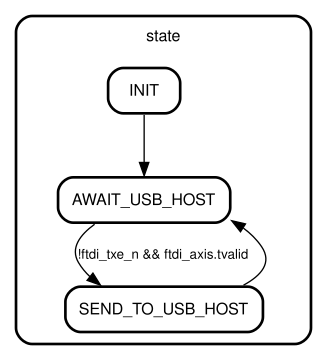
\includegraphics[width=\textwidth/3]{figures/ft232h-state-machine.png}
  \caption{FT322H AXI Wrapper State Machine}
  \label{fig:ft232h-state-machine}
\end{figure}

The state machine Waits for the AXI stream to have data available and for the
FT232HQ to be ready for new data. When this condition is satisfied, the byte is
sent out and the state machine automatically transitions back to the await
state.

It should also be noted that there is a comment in the code above indicating
that the \code{sys_axis} stream input must be changed based on whether you want
to use the XADC or high-speed ADC data. In this case, the XADC is used.

\subsubsection{XADC IP Core}
Shown below is the XADC IP core used to extract data from the internal XADC on
the FPGA. This IP core is made custom using the XADC Wizard tool in Xilinx
Vivado. The core is configured to only output the two FPGA ADC channels in use
on the TeachEE PCB via a Dynamic Reconfiguration Port (DRP) interface. The DRP
signals are then fed into an AXIS adapter module for interface standardization.

\setstretch{1}
\begin{minted}{systemverilog}
    xadc_teachee xadc_teachee_inst (
        // Clock and Reset
        .dclk_in(sys_clk),          // input wire dclk_in
        .reset_in(reset),        // input wire reset_in

        // DRP interface
        .di_in(0),              // input wire [15 : 0] di_in
        .daddr_in(xadc_daddr),        // input wire [6 : 0] daddr_in
        .den_in(xadc_den),            // input wire den_in
        .dwe_in(0),            // input wire dwe_in
        .drdy_out(xadc_drdy),        // output wire drdy_out
        .do_out(xadc_do),            // output wire [15 : 0] do_out

        // Dedicated analog input channel (we do not use this)
        .vp_in(0),              // input wire vp_in
        .vn_in(0),              // input wire vn_in

        // analog input channels, vaux4 is pin 15 = VIOUT of current sensor
        // vaux12 is pin 16 = low speed voltage channel.
        .vauxp4(xa_p[0]),            // input wire vauxp4
        .vauxn4(xa_n[0]),            // input wire vauxn4
        .vauxp12(xa_p[1]),          // input wire vauxp12
        .vauxn12(xa_n[1]),          // input wire vauxn12

        // conversion status signals
        .channel_out(),  // output wire [4 : 0] channel_out
        .eoc_out(),          // output wire eoc_out
        .alarm_out(),      // output wire alarm_out
        .eos_out(xadc_eos),          // output wire eos_out
        .busy_out()        // output wire busy_out
    );
\end{minted}
\setstretch{2}

\subsubsection{ADC AXIS Wrappers}
Similarly to the \code{ft232h} module, both the XADC and high-speed ADC have
AXIS wrapper modules. Both wrapper modules function in the same manner, they
await new data from the ADC and place it in AXIS compliant FIFO queue. The
\code{sample_stream} output is internally connected to this queue where samples
can be consumed by the FT232HQ. Given below is the instantiation of both
modules.
\setstretch{1}
\begin{minted}{systemverilog}
    xadc_drp_addr_t xadc_daddr;
    var logic xadc_den;

    var logic xadc_drdy;
    var logic[XADC_DRP_DATA_WIDTH-1:0] xadc_do;
    var logic xadc_eos;

    xadc_drp_axis_single_stream xadc_drp_axis_adapter_inst (
        .xadc_dclk(sys_clk),
        .xadc_reset(reset),

        // DRP and Conversion Signals
        .xadc_daddr(xadc_daddr),
        .xadc_den(xadc_den),
        .xadc_drdy(xadc_drdy),
        .xadc_do(xadc_do),

        .xadc_eos(xadc_eos),

        .sample_stream(xadc_sample_channel.Source)
    );

    hsadc_axis_wrapper hsadc (
        .sample_clk(clk_10),
        .stream_clk(sys_clk),
        .reset(reset),

        .hsadc_ctrl_signals(hsadc_ctrl.sink),
        .sample_stream(hsadc_sample_channel.source)
    );

\end{minted}
\setstretch{2}

The XADC wrapper takes in the DRP control signals from the XADC IP core and the
high-speed ADC wrapper gets all the control signals from a single interface
declared earlier in the file.


\subsubsection{AXIS and Verilog AXIS} \label{sec:external-fpga-libs} AXIS, also
referred to as AXI Stream is the standard protocol used throughout the FPGA
datapath. While there are many signals in an AXI interface, the primary signals
are called \code{tdata}, \code{tready}, \code{tvalid}. Only when \code{tready}
and \code{tvalid} are asserted can you consume data from the \code{tdata} bus.
\code{tready} is controlled by the receiver so it can regulate the rate at which
it consumes data while \code{tvalid} is controlled by the sender to tell the
receiver when new data is ready on the \code{tdata} lines. The full
specification contains many additional signals but these are the three that most
often being manipulated during data transmission \cite{axis_spec}. Figures
\ref{fig:axis-read} \ref{fig:axis-write} show the AXIS read and write timing
diagrams respectively.

\begin{figure}[H]
  \centering
  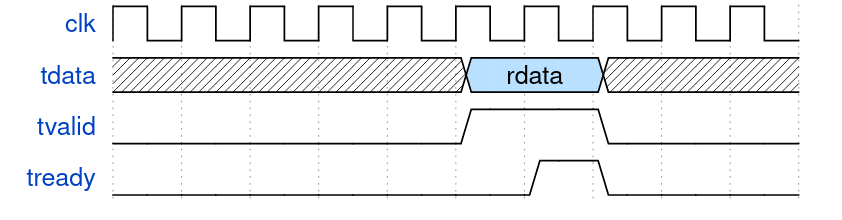
\includegraphics[width=\textwidth]{figures/axis_read.png}
  \caption{AXIS Read Transaction Timing Diagram}
  \label{fig:axis-read}
\end{figure}

In AXIS read and write transactions, the producer is responsible for
\code{tdata} and \code{tvalid} signals while the consumer toggles \code{tready}.
This allows the consumer to know when new data becomes available and it is able
to signal to the producer when it is ready to accept it via \code{tready}. All
three signals should only be asserted or deasserted in synchronization with the
system clock per the specification. As shown in Figure \ref{fig:axis-read},
\code{tvalid} is asserted on the same rising edge as the new data coming onto
the \code{tdata} bus. The consumer sees this and asserts tready on the next
rising edge consuming the data. In the case where multiple words of data are
queued by the producer, the \code{tdata} value will advance to the next byte
available after each cycle where both \code{tvalid \&\& tready} is true. This
allows a new read to take place every cycle if the producer has the data and the
consumer is ready for it. This simple protocol yields strong performance and
flexibility with minimal FPGA LUT resources used. It should be noted that for
any AXIS transaction to take place \code{tready \&\& tvalid} must be true.

\begin{figure}[H]
  \centering
  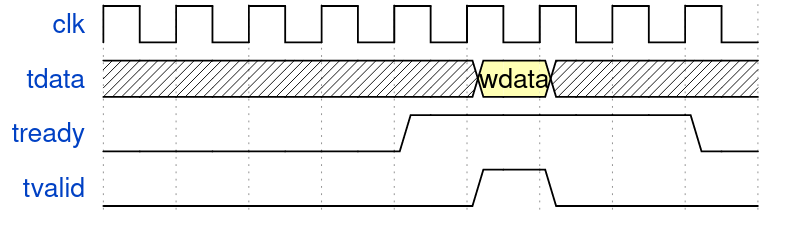
\includegraphics[width=\textwidth]{figures/axis_write.png}
  \caption{AXIS Write Transaction Timing Diagram}
  \label{fig:axis-write}
\end{figure}

In the AXIS write case shown in Figure \ref{fig:axis-write}, the consumer first
asserts \code{tready}, which tells the producer that it can accept new data.
Once the producer has data, it asserts the value on \code{tdata} and drives
\code{tvalid} high on the same rising edge. Since \code{tready \&\& tvalid} is
true, the data is written to the consumer successfully. This design pattern is
replicated repeatedly throughout the FPGA codebase provided in Appendix
\ref{appendix:rtl-code}.

In addition to the simplicity protocol, there is significant library support for
AXI streams. In the case of TeachEE, the \code{verilog-axis} library is used
\cite{verilog_axis_lib}. This library contains a variety of useful verilog
modules, all of which expose an AXIS interface at their inputs and outputs. The
standard interface across all modules makes connecting up the library modules
with TeachEE modules trivial. The only modification made to these library
modules was to wrap them in another more ergonomic module. Since the library is
written in Verilog, it does not have access to interfaces, which are a feature
of SystemVerilog only. As a result, each AXIS signal is written out individually
making instanciating and connecting the modules unwieldy. In order to bundle all
these signals into one module port, the \code{axis_interface} is used. For each
module in the \code{verilog-axis} library used by TeachEE, a wrapper module is
written that places all the signals for the AXI streams in AXIS interfaces
making module connectivity far simpler thanks to SystemVerilog. This is possible
due to the Xilinx Vivado project build configuration that cross compiles both
Verilog and SystemVerilog. The interface is also designed to seamlessly handle
the producer and consumer cases discussed above using modports. The
\code{Source} modport can be used on producer stream interfaces and the
\code{Sink} modport can be used for consumers. The modports switch the direction
of the signals from \code{input} to \code{output} depending on the use case.

\code{verilog-axis} contains many modules but there are three that were employed
when writing the RTL code for TeachEE. 

The first module is \code{axis_async_fifo}, which is wrapped by
\code{axis_async_fifo_wrapper}. This module constructs a First-In-First-Out
(FIFO) Queue and is used repeatedly throughout the code. The first and foremost
purpose of the Queue is to provide sample memory to ensure samples are not
dropped when the rate of production deviates from the rate of consumption.
Secondly the FIFO is asynchronous, meaning it can use different clock signals
for its input and output. The module has internal synchronization logic to bring
data across clock domains. This functionality was critical in the TeachEE RTL
design as we had multiple clock domains and needed to transfer data between them
efficiently. The top-level system, USB FIFO, HSADC, and XADC all had different
clock signals and had their data inputs buffered by asynchronous FIFOs.

The second key module is the \code{axis_adapter}, which is wrapped by
\code{axis_adapter_wrapper}. This module takes an AXI Stream, and adapts it to a
smaller width specified as a parameter in the module instantiation. This module
was critical in getting the 32-bit sample stream from the XADC to fit the 8-bit
stream accepted by the USB FIFO.

The final module used from the library was the \code{cobs_encode}, which is
wrapped by \code{cobs_encode_wrapper}. This module takes an 8-bit input stream
and outputs the same data encoded using Consistent Overhead Byte Stuffing
(COBS). The COBS encoder is highly efficient and only creates two additional
bytes of overhead ensuring the USB link bandwidth is not wasted \cite{cobs}.
In order to transmit samples to the computer, the 32-bit stream from the XADC
(or 16-bit from the HSADC) is adapted to 8 bits using \code{axis_adapter}. The
resulting 8-bit stream is fed into the COBS encoder, whose output is connected
to the USB FIFO. These two modules make up the packet encoding stack.

Perhaps the most important benefit of AXIS over other streaming interfaces is
its direct compatibility with the more fully-featured AXI bus. AXI is a standard
memory-mapped bus interface used in ARM processors \cite{axi_spec}. Since all
modules in TeachEE's FPGA codebase use AXI streams, the platform is highly
extensible and can be connected to ARM coprocessors with minimal effort. Such a
design extension would make TeachEE similar architecturally to more expensive
benchtop oscilloscopes that make use of both an ASIC and traditional processor
through a high-speed interconnection protocol. An example of this architecture
is Keysight's MegaZoom ASIC \cite{keysight_megazoom}.

\subsection{Software} % ERIC
% Basically everything from poster with more detail

\section{Testing, Evaluation \& Verification} \label{sec:testing}
The following tables outline the target hardware and software specifications of
this project.
\subsection{PCB Verification} % ETHAN
% Hardware tests
\subsection{FPGA Verification} % ETHAN
% Talk about FPGA automated sims, testbenches CI ETC
\subsection{Software Verification} % ERIC
% Rust CI, Testing with mock byte streams? 
\subsection{System Level Verification} % ETHAN / ERIC
% This subsection should include some notes on time spent in the lab running all
% three HW, FPGA and SW components integrated together. Also comparing our
% output against that of a real scope connected to the same signal

\section{Project Planning and Budgeting} % ERIC

\section{Stakeholder Needs} % John / Tim
%% Describe how you considered stakeholder needs in your design, and how factors
%% like safety, privacy, codes/standards, manufacturability, ethics and cost were
%% considered in your design.

% JOHN should use this section to discuss why our device is more suited to EE
% undergrads than what is currently on the market. Tim should provide some input
% on manufacturability and cost too.

\section{Compliance with System Requirements} % John
%% Compliance with specifications – Include your original specifications table from
%% the Blueprint and add extra column to it as shown below and report what you
%% obtained with your final design. If any of your specs were not achieved or fell
%% outside the tolerance values, explain why in this section. Your mark for this
%% section depends on how close you got to your specs

\section{Conclusions \& Recommendations} % Tim
%% Conclusions and recommendations – provide commentary on the main technical
%% lessons learned from this project; is there potential for lasting impact for
%% this project beyond this course? Can more research be done in an area? Should
%% someone tackle this problem again but using a different approach? Is there
%% potential for commercialization? If this were to be scaled out to a commercial
%% version how would it be manufactured and what would the cost be? Speculate about
%% the market size for such a product. If the product makes it to the market, what
%% are the potential positive and adverse societal and cultural impacts of the
%% product? How can the adverse impacts be mitigated?

\section{Overall Team Effort}
The following table quantifies the percentage effort each team member expended
on all aspects of the project.

\begin{table}[H]
  \caption{Team Effort Table}
  \centering
  \begin{tabularx}{10cm}{l|l}
    \textbf{Name} & \textbf{Effort Expended \%}\\
    \hline
    Ethan Peterson & TODO \\
    \hline
    Eric Yang & TODO \\
    \hline
    Timothy Morland & TODO \\
    \hline
    John Giorshev & TODO \\
  \end{tabularx} 
\end{table}
\newpage

\bibliographystyle{IEEEtran}
\bibliography{report}

\newpage
\setstretch{1}

\pagestyle{empty}

    \begin{appendices}
        \begin{landscape}
        \section{Schematics}
        \label{appendix:schematic}
    \centering
    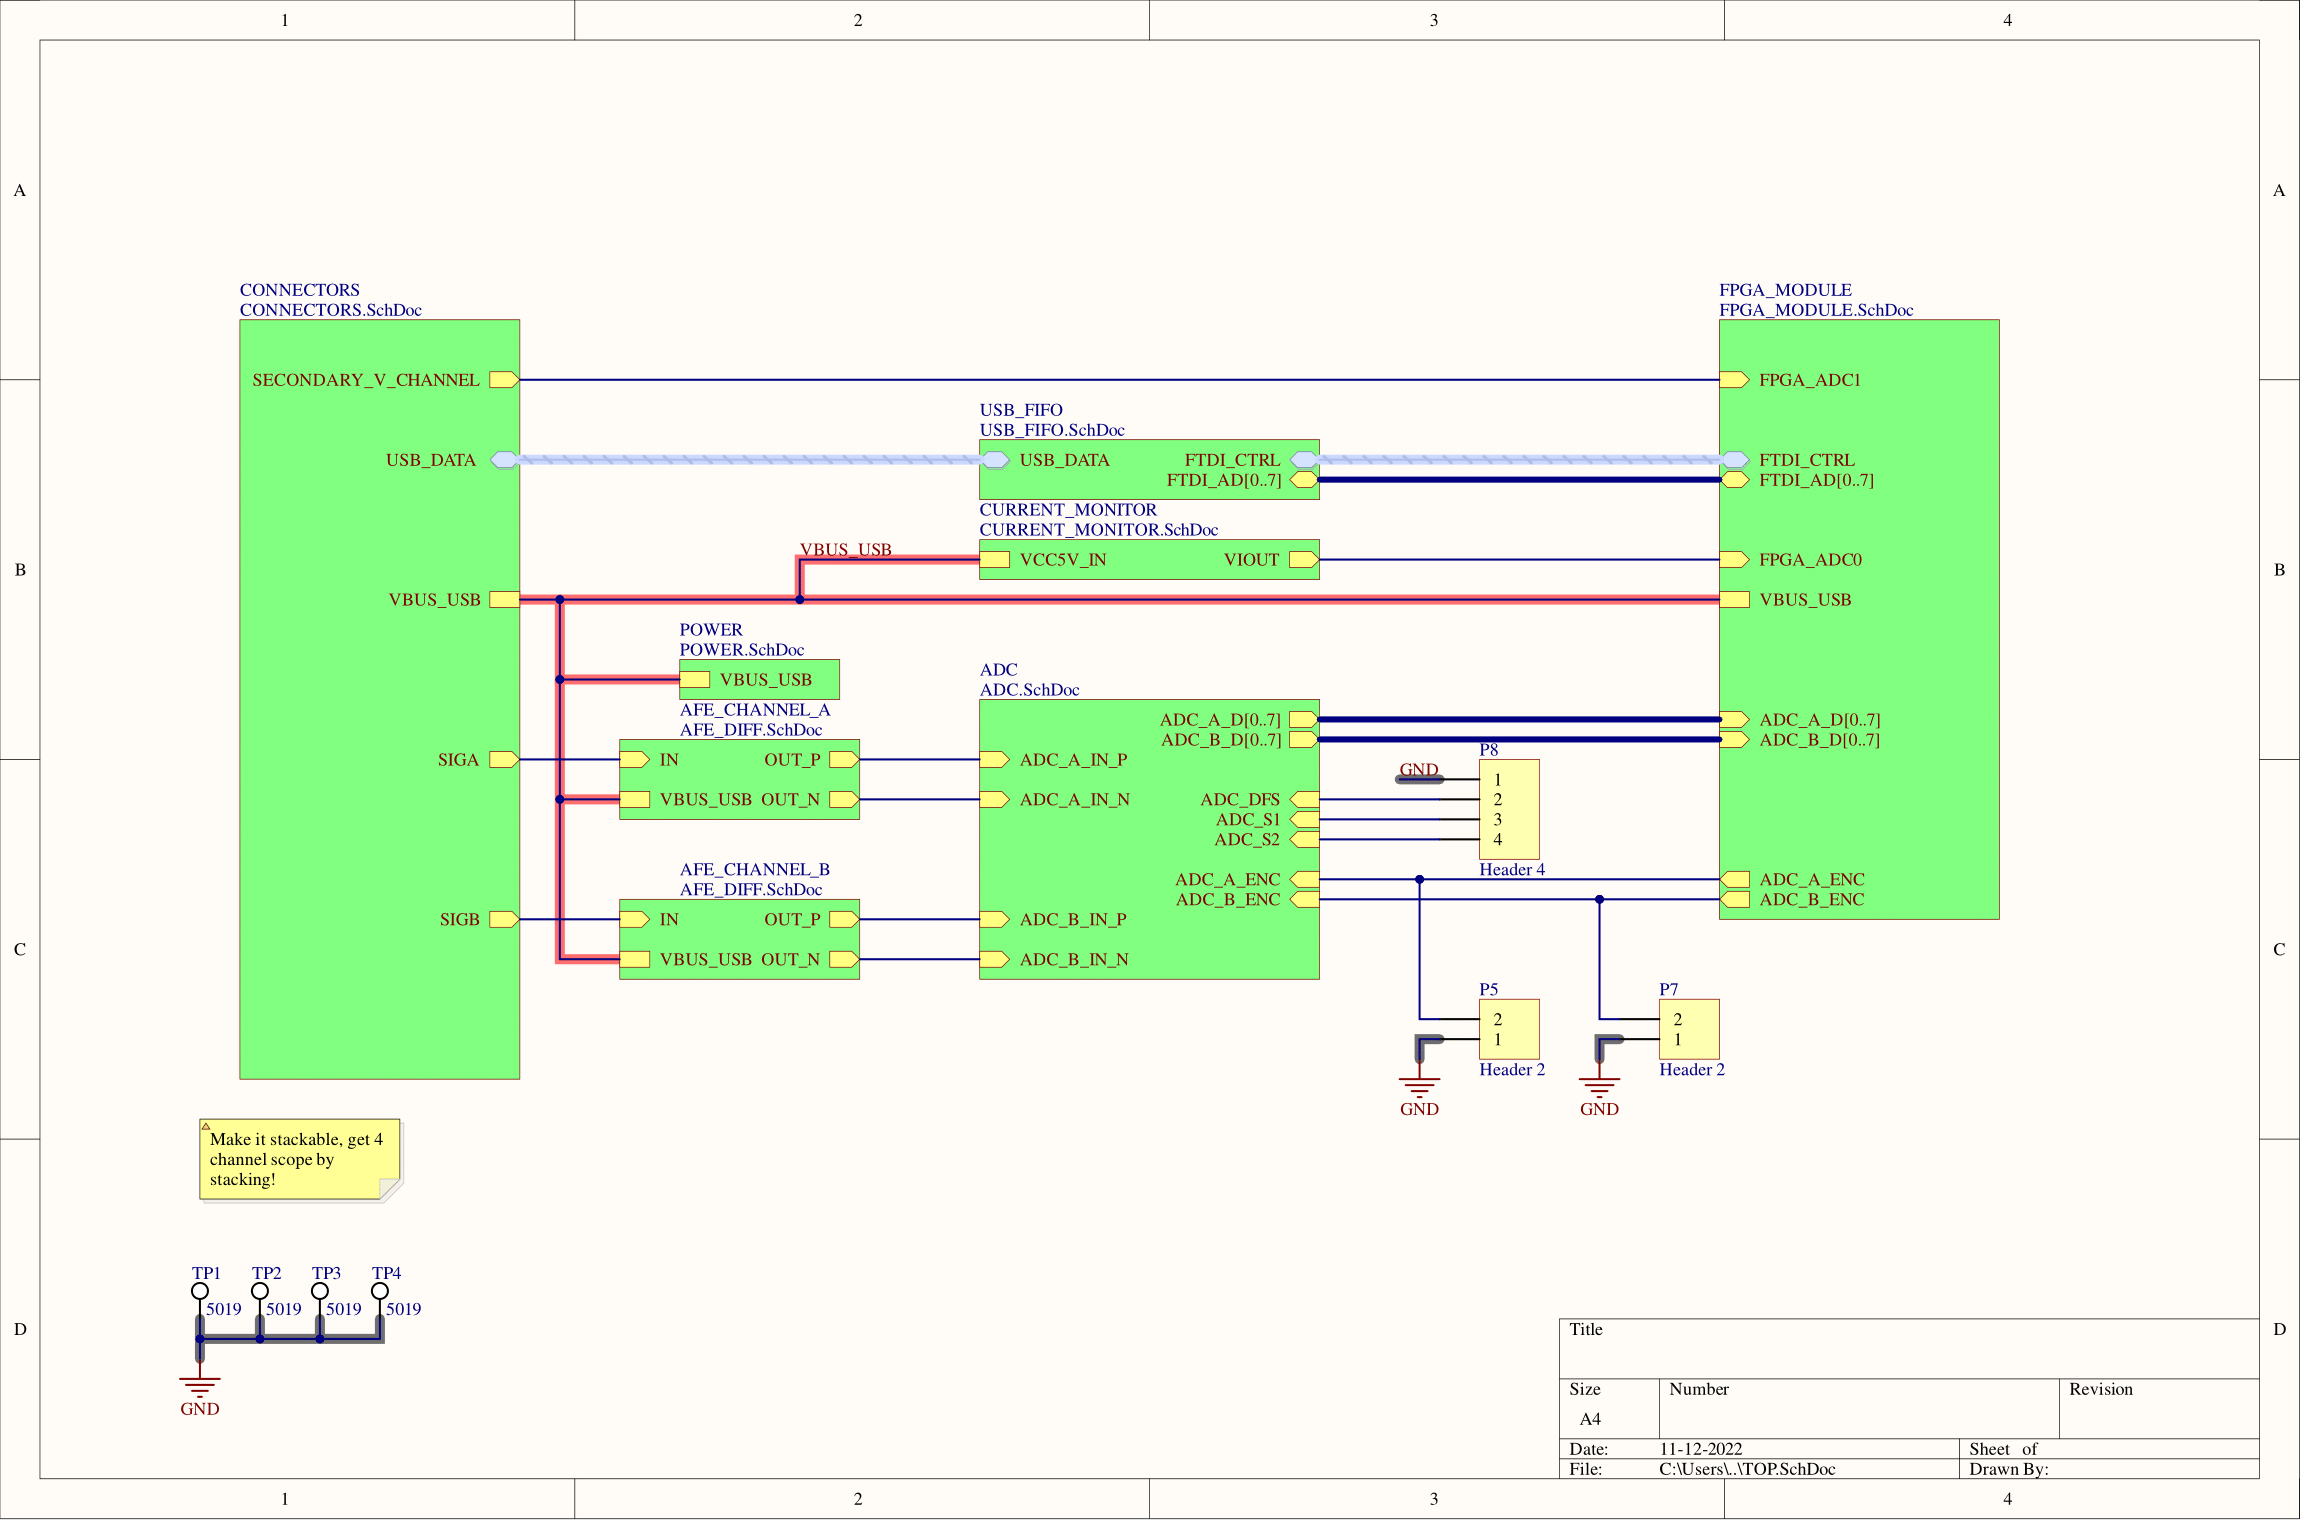
\includegraphics[height=15cm]{schematics/schematic1-1.png}
        \end{landscape}
    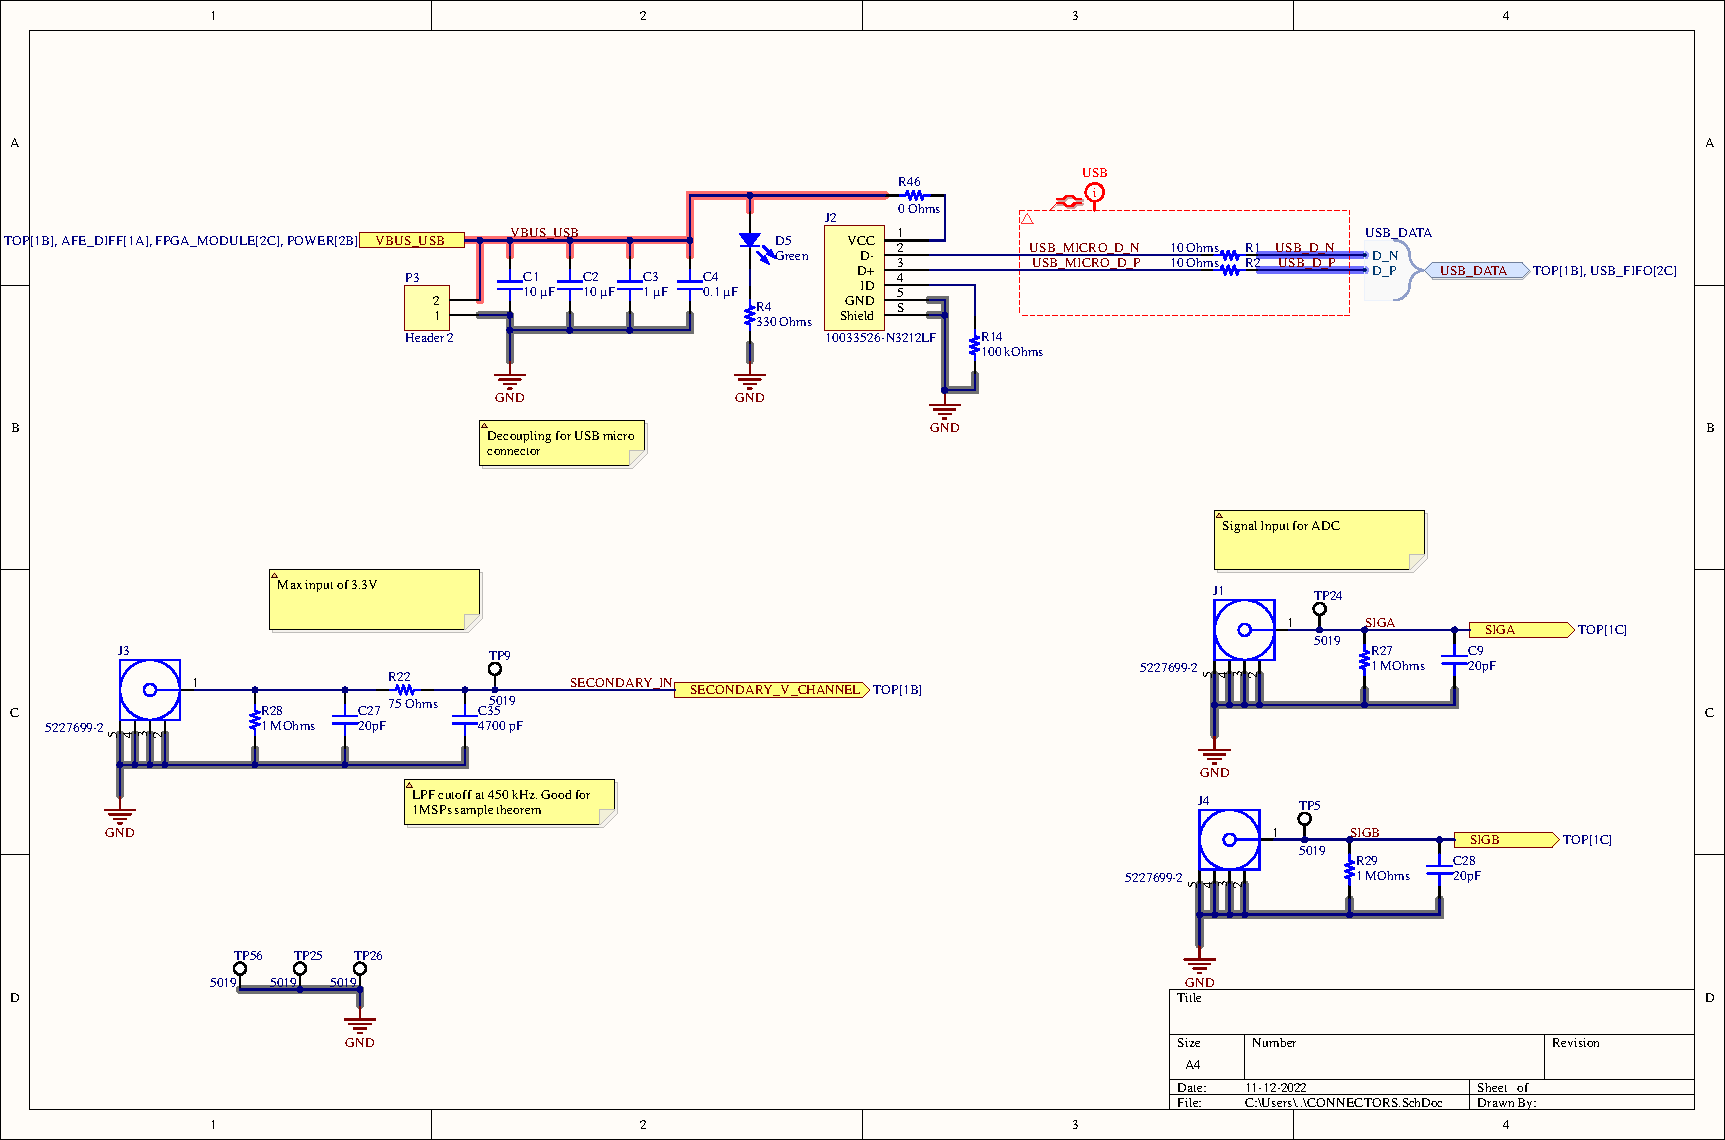
\includepdf[pages=-,landscape=true]{schematics/schematic2-8.pdf}

        \begin{landscape}
        \section{PCB Layout}
        \label{appendix:layout}
    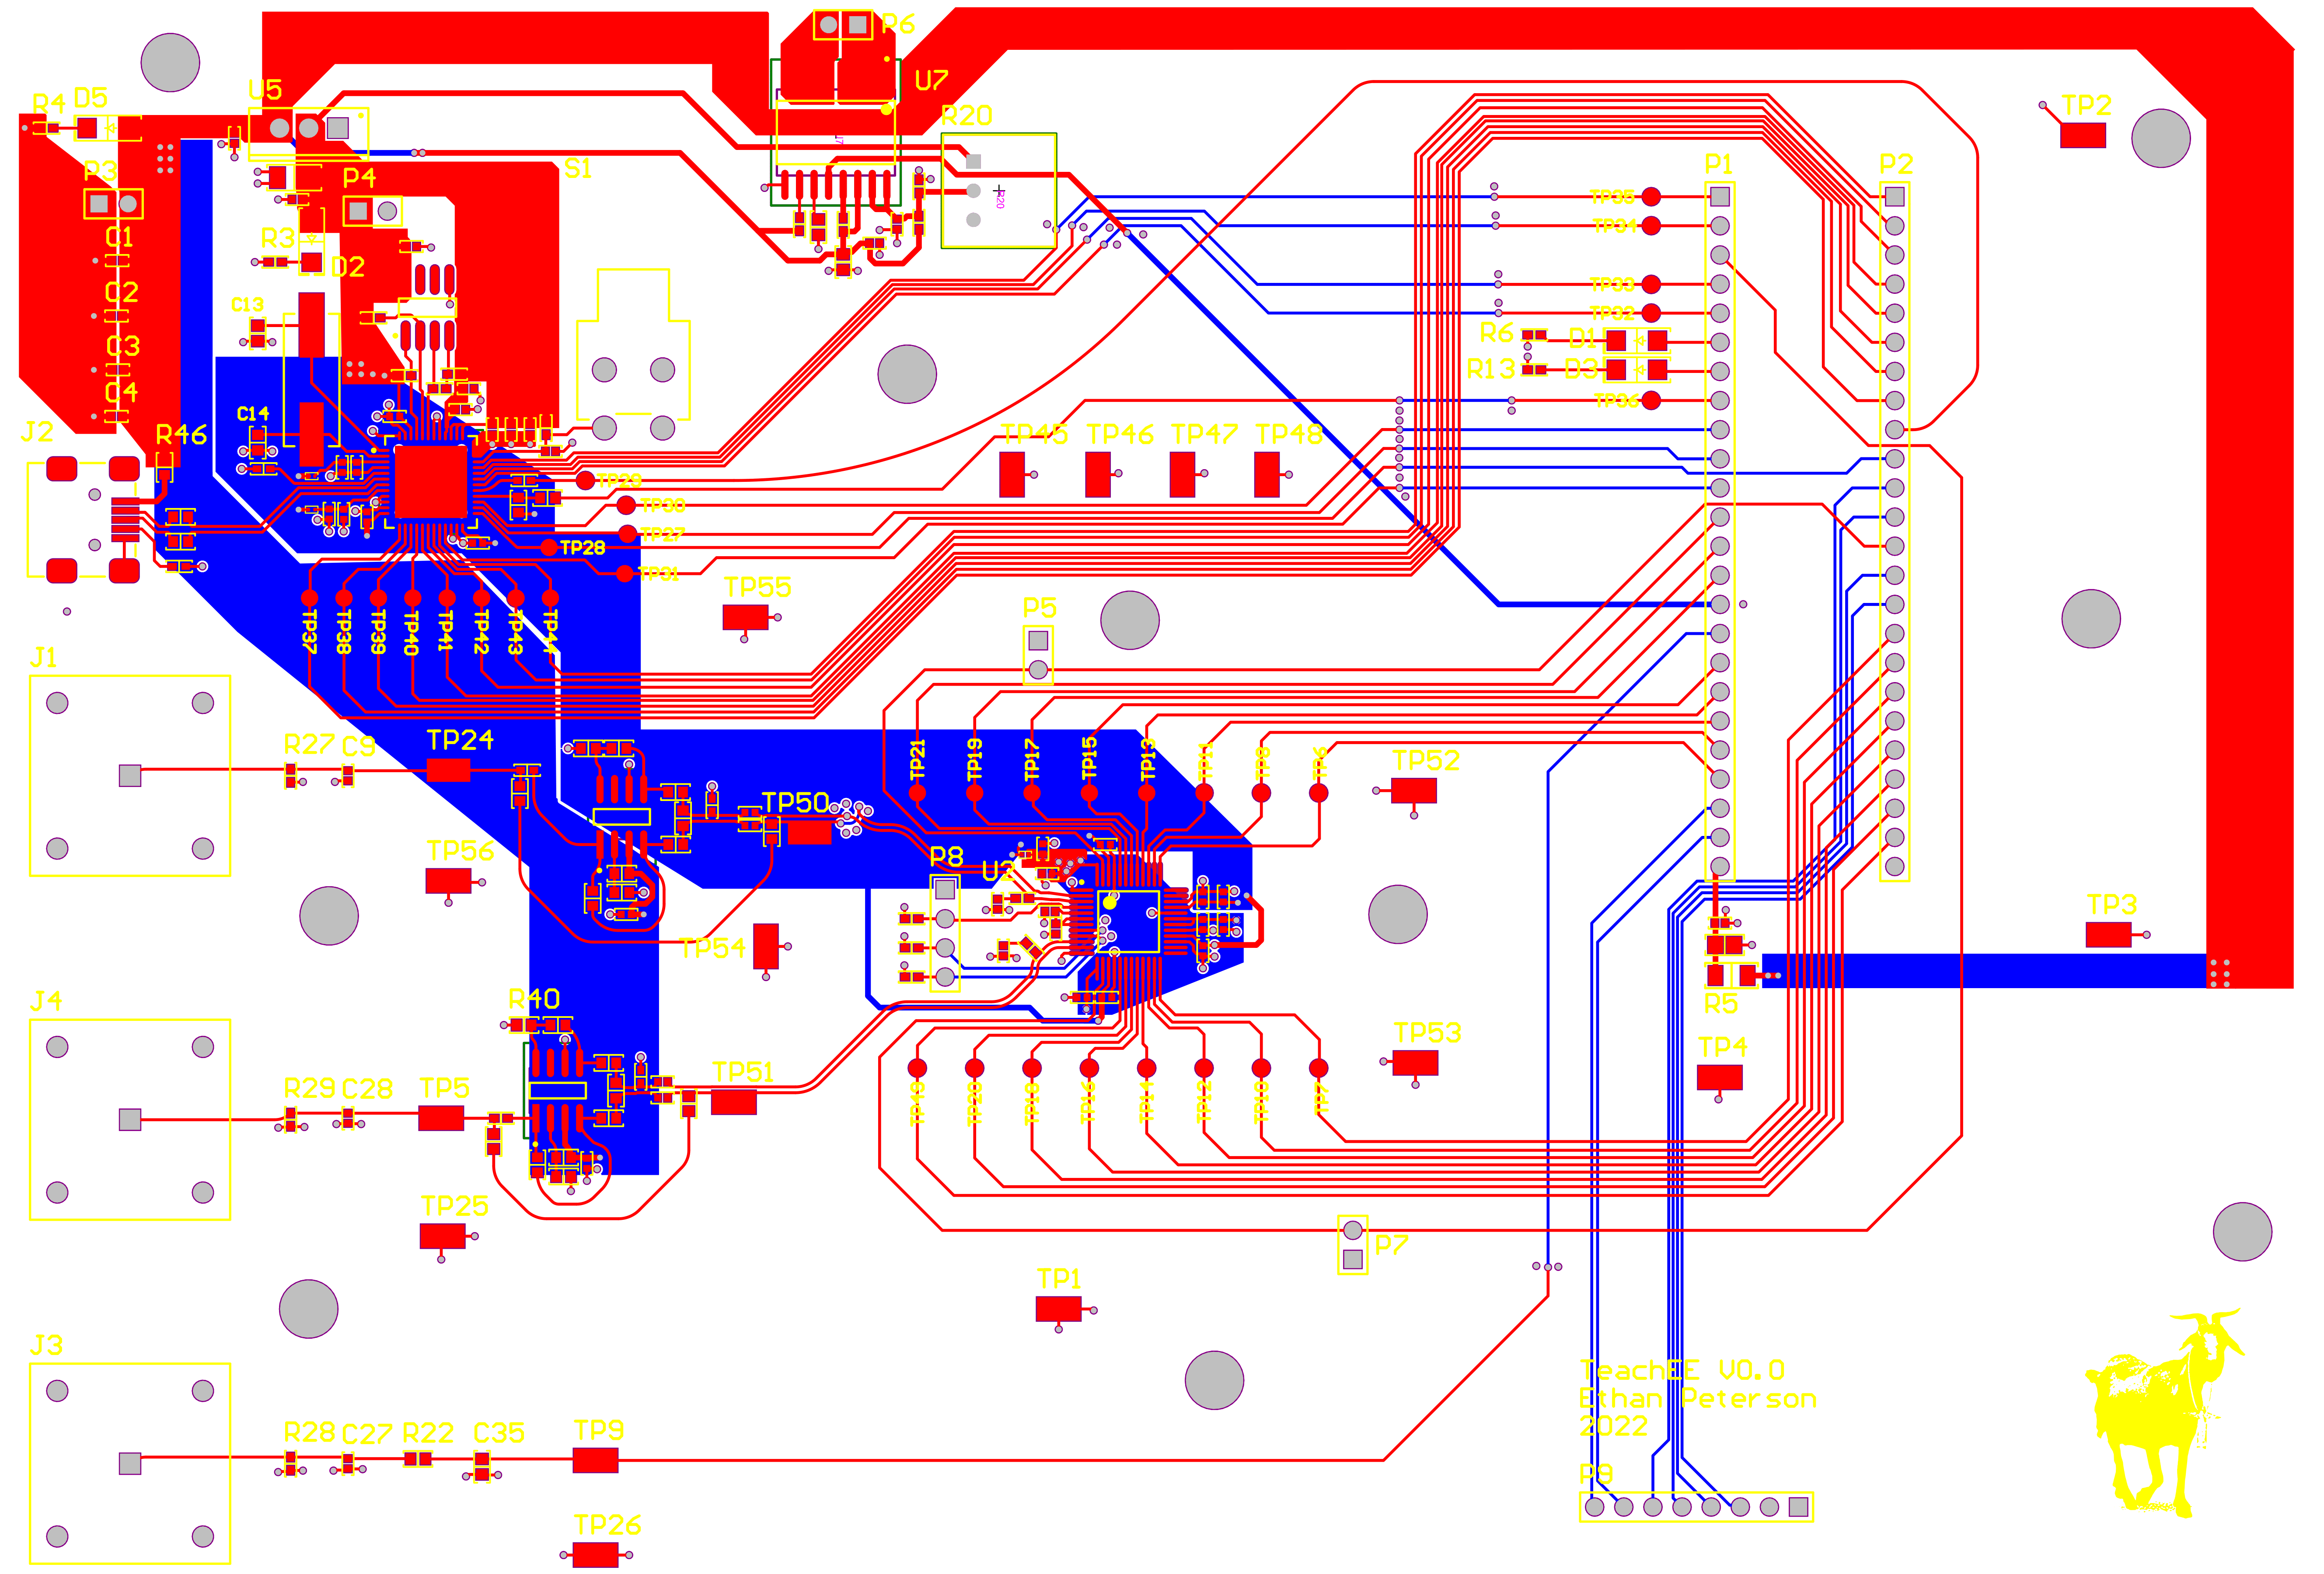
\includegraphics[height=15cm]{schematics/Layout.png}
        \end{landscape}

        \section{PCB Bill of Materials}
        \label{appendix:bom}
    \begin{table}[H]
    \begin{tabular}{p{1.7in}|p{0.3in}|p{0.8in}|p{0.7in}|p{0.7in}|p{1in}}
        \textbf{Designator} & \textbf{QTY} & \textbf{Description} & \textbf{Comment} & \textbf{Footprint} & \textbf{Part Number} \\ \hline 
        C1, C2, C37, C48 & 4 & CAP CER 10UF 10V X5R 0402 & 10 µF & CAP 0402\_1005 & CL05A106MP8NUB8 \\ \hline
        C3 & 1 & CAP CER 1UF 10V X7S 0402 & 1 µF & CAP 0402\_1005 & GRM155C71A105KE11D \\ \hline
        C4, C11, C16, C17, C18, C19, C20, C21, C22, C24, C26, C29, C30, C38, C39, C40, C41, C42, C43, C44, C45, C46, C47, C50\_AFE\_CHANNEL\_A, C50\_AFE\_CHANNEL\_B, C52\_AFE\_CHANNEL\_A, C52\_AFE\_CHANNEL\_B, C53\_AFE\_CHANNEL\_A, C53\_AFE\_CHANNEL\_B & 29 & CAP CER 0.1UF 50V X5R 0402 & 0.1 µF & CAP 0402\_1005 & CGA2B3X5R1H104M050BB \\ \hline
        C5, C12, C32, C34 & 4 & CAP CER 0.1UF 10V X7R 0402 & 0.1µF & CAP 0402\_1005 & 0402ZC104KAT2A \\ \hline
        C6 & 1 & CAP CER 10UF 16V X5R 1206 & 10 µF & CAP 1206\_3216 - 0.8MM & EMK316BJ106MD-T \\ \hline
        C7 & 1 & CAP CER 10UF 35V X6S 0805 & 10 µF & CAP 0805\_2012 & GRM21BC8YA106KE11L \\ \hline
        C8, C15, C23, C25 & 4 & CAP CER 4.7UF 16V X5R 0402 & 4.7 µF & CAP 0402\_1005 & CL05A475MO5NUNC \\ \hline
        C9, C27, C28 & 3 & CAP CER 20PF 25V NP0 0402 & 20pF & CAP 0402\_1005 & 04023U200JAT2A \\ \hline
    \end{tabular}
    \end{table}

    \newpage

    \begin{table}[H]
    \begin{tabular}{p{1.7in}|p{0.3in}|p{0.8in}|p{0.7in}|p{0.7in}|p{1in}}
        \textbf{Designator} & \textbf{QTY} & \textbf{Description} & \textbf{Comment} & \textbf{Footprint} & \textbf{Part Number} \\ \hline 
        C10 & 1 & CAP MLCC 0.01UF 100V X7R 0402 & 10000 pF & CAP 0402\_1005 & HMK105B7103KVHFE \\ \hline
        C13, C14 & 2 & CAP CER 36PF 100V NP0 0603 & 36pF & CAP 0603\_1608 & 06031A360JAT2A \\ \hline
        C31 & 1 & CAP CER 1UF 16V X7R 0603 & 1 µF & CAP 0603\_1608 & C0603C105K4RACAUTO \\ \hline
        C33, C35 & 2 & CAP CER 0603 4.7NF 16V X7R 10\% & 4700 pF & CAP 0603\_1608 & C0603C472K4RECAUTO \\ \hline
        C51\_AFE\_CHANNEL\_A, C51\_AFE\_CHANNEL\_B & 2 & CAP CER 15PF 25V C0G/NP0 0603 & 15 pF & CAP 0603\_1608 & C0603C150J3GACAUTO \\ \hline
        D1, D3 & 2 & LED SMD & Blue & LED 1206\_3216 BLUE & APTL3216QBC/D-01 \\ \hline
        D2, D5 & 2 & LED SMD & Green & LED 1206\_3216 GREEN & APTL3216ZGCK-01 \\ \hline
        FB1, FB2, FB3 & 3 & FERRITE BEAD 33 OHM 0201 1LN & 33 Ohms @ 100 MHz & FER 0201\_0603 & MMZ0603F330CT000 \\ \hline
        J1, J3, J4 & 3 & Jack BNC Connector, 1 Position, Height 16.26 mm, Tail Length 6.35 mm, -55 to 85 degC, RoHS, Tube & 5227699-2 & & 5227699-2 \\ \hline
        J2 & 1 & CONN RCPT MINI USB B 5POS SMD RA & & & 10033526-N3212LF \\ \hline
    \end{tabular}
    \end{table}
    \newpage
    \begin{table}[H]
        \begin{tabular}{p{1.7in}|p{0.3in}|p{0.8in}|p{0.7in}|p{0.7in}|p{1in}}
        \textbf{Designator} & \textbf{QTY} & \textbf{Description} & \textbf{Comment} & \textbf{Footprint} & \textbf{Part Number} \\ \hline 
        R1, R2 & 2 & RES SMD 10 OHM 0.1\% 1/10W 0603 & 10 Ohms & RES 0603\_1608 & CRT0603-BY-10R0ELF \\ \hline
        R3, R6, R13 & 3 & RES 220 OHM 1\% 1/8W 0402 & 220 Ohms & RES 0402\_1005 & CRGP0402F220R \\ \hline
        R4 & 1 & RES SMD 330 OHM 5\% 1/16W 0402 & 330 Ohms & RES 0402\_1005 & AC0402JR-07330RL \\ \hline
        R5 & 1 & 1206 40 AMP JUMPER & 0 Ohms & RES 1206\_3216 & JR1206X40E \\ \hline
        R7 & 1 & RES SMD 12K OHM 0.1\% 1/16W 0402 & 12 kOhms & RES 0402\_1005 & CPF0402B12KE1 \\ \hline
        R8, R9, R10, R11, R17, R18, R19, R21, R32, R33, R34 & 11 & RES 10K OHM 0.1\% 1/10W 0402 & 10 kOhms & RES 0402\_1005 & RP73PF1E10KBTD \\ \hline
        R12 & 1 & RES 1.8K OHM 1\% 1/16W 0402 & 1.8 kOhms & RES 0402\_1005 & RC0402FR-071K8L \\ \hline
        R14 & 1 & RES SMD 100K OHM 0.1\% 1/16W 0402 & 100 kOhms & RES 0402\_1005 & CPF0402B100KE \\ \hline
        R15, R46 & 2 & RES SMD 0 OHM JUMPER 1/2W 0603 & 0 Ohms & RES 0603\_1608 & 5110 \\ \hline
        R22 & 1 & RES SMD 75 OHM 1\% 1/10W 0603 & 75 Ohms & RES 0603\_1608 & AC0603FR-0775RL \\ \hline
        R26 & 1 & RES 24 OHM 1\% 1/16W 0402 & 24 Ohms & RES 0402\_1005 & RC0402FR-0724RL \\ \hline
        \end{tabular}
    \end{table}
    \newpage
    \begin{table}[H]
        \begin{tabular}{p{1.7in}|p{0.3in}|p{0.8in}|p{0.7in}|p{0.7in}|p{1in}}
        \textbf{Designator} & \textbf{QTY} & \textbf{Description} & \textbf{Comment} & \textbf{Footprint} & \textbf{Part Number} \\ \hline 
        R27, R28, R29 & 3 & RES 1M OHM 1\% 1/16W 0402 & 1 MOhms & RES 0402\_1005 & RMCF0402FT1M00 \\ \hline
        R36\_AFE\_CHANNEL\_A, R36\_AFE\_CHANNEL\_B & 2 & RES SMD 523 OHM 0.1\% 1/16W 0402 & 523 Ohms & RES 0402\_1005 & ERA-2ARB5230X \\ \hline
        R37\_AFE\_CHANNEL\_A, R37\_AFE\_CHANNEL\_B, R40\_AFE\_CHANNEL\_A, R40\_AFE\_CHANNEL\_B, R41\_AFE\_CHANNEL\_A, R41\_AFE\_CHANNEL\_B & 6 & RES SMD 500 OHM 0.05\% 1/10W 0603 & 500 Ohms & RES 0603\_1608 & TNPU0603500RAZEN00 \\ \hline
        R39\_AFE\_CHANNEL\_A, R39\_AFE\_CHANNEL\_B, R43\_AFE\_CHANNEL\_A, R43\_AFE\_CHANNEL\_B & 4 & RES 50 OHM 5\% 1/8W 0603 & 50 Ohms & RES 0603\_1608 & CH0603-50RJNTA \\ \hline
        R42\_AFE\_CHANNEL\_A, R42\_AFE\_CHANNEL\_B & 2 & RES SMD 4.02K OHM 1\% 1/10W 0603 & 4.02 kOhms & RES 0603\_1608 & AC0603FR-074K02L \\ \hline
        R44\_AFE\_CHANNEL\_A, R44\_AFE\_CHANNEL\_B & 2 & RES SMD 1K OHM 1\% 1/10W 0603 & 1 kOhms & RES 0603\_1608 & AA0603FR-071KL \\ \hline
        R45\_AFE\_CHANNEL\_A, R45\_AFE\_CHANNEL\_B & 2 & RES 25 OHM 0.1\% 1/20W 0402 & 25 Ohms & RES 0402\_1005 & FC0402E25R0BST0 \\ \hline
        S1 & 1 & SWITCH PUSH SPST-NO 0.4VA 28V & &  & AB11AH-HA \\ \hline
        TP1, TP2, TP3, TP4, TP5, TP9, TP24, TP25, TP26, TP45, TP46, TP47, TP48, TP50, TP51, TP52, TP53, TP54, TP55, TP56 & 20 & Test Point, 1 Position SMD, RoHS, Tape and Reel & 5019 & KSTN5019 & 5019 \\ \hline
        U1 & 1 & IC HS USB TO UART/FIFO 48QFN & FT232 & QFN-48 & FT232HQ-REEL \\ \hline
        \end{tabular}
    \end{table}
    \newpage
    \begin{table}[H]
        \begin{tabular}{p{1.7in}|p{0.3in}|p{0.8in}|p{0.7in}|p{0.7in}|p{1in}}
        \textbf{Designator} & \textbf{QTY} & \textbf{Description} & \textbf{Comment} & \textbf{Footprint} & \textbf{Part Number} \\ \hline 
        U2 & 1 & Dual 8-Bit AD Converter with Parallel Interface, 40MSPS, -40 to +85 degC, ST-48, Pb-Free, Tray &  & ST-48M & AD9288BSTZ-40 \\ \hline
        U3\_AFE\_CHANNEL\_A, U3\_AFE\_CHANNEL\_B & 2 & IC ADC DRIVER 8SOIC & AD8138 & R-8-IPC\_A & AD8138ARZ-R7 \\ \hline
        U5 & 1 & Fixed Low Drop Positive Voltage Regulator, 3.3V, 3-Pin TO-220 & LD1117 & TO220 & LD1117V33C \\ \hline
        U6 & 1 & 2K, 128x16-bit, 2.5V Microwire Serial EEPROM, 8-Pin SOIC 150mil, Commercial Temperature, Tape and Reel & 93LC56 & SOIC8 & 93LC56BT/SN \\ \hline
        U7 & 1 & CURRENT SENSOR & ACS720 &  & ACS720KLATR-15AB-T \\ \hline
        Y1 & 1 & CRYSTAL 12.0000MHZ 20PF SMD & 12 MHz & ABLS & ABLS-12.000MHZ-20-B-3-H-T \\ \hline
        \end{tabular}
    \end{table}

    % TODO: needs smaller font size or line wrapping
    \section{TeachEE SystemVerilog RTL Code} \label{appendix:rtl-code}
    This appendix contains all the SystemVerilog RTL files in the TeachEE
    project. Each subsection corresponds to the files in a particular folder of
    the GitHub repository.

    \subsubsection{TeachEE Main Project Top Level Module}
    \inputminted[linenos,breaklines]{systemverilog}{../../rtl/teachee/teachee.sv}

    \subsection{AXIS} \label{appendix:axis}
    \subsubsection{axis\_adapter\_wrapper.sv}
    \inputminted[linenos,breaklines]{systemverilog}{../../rtl/axis/axis_adapter_wrapper.sv}
    \subsubsection{axis\_async\_fifo\_wrapper.sv}
    \inputminted[linenos,breaklines]{systemverilog}{../../rtl/axis/axis_async_fifo_wrapper.sv}
    \subsubsection{axis\_interface.sv} \label{appendix:axis-interface}
    \inputminted[linenos,breaklines]{systemverilog}{../../rtl/axis/axis_interface.sv}

    \subsection{COBS}
    \subsubsection{cobs\_axis\_adapter\_wrapper.sv}
    \inputminted[linenos,breaklines]{systemverilog}{../../rtl/cobs/cobs_axis_adapter_wrapper.sv}
    \subsubsection{cobs\_encode\_wrapper.sv}
    \inputminted[linenos,breaklines]{systemverilog}{../../rtl/cobs/cobs_encode_wrapper.sv}

    \subsection{FT232H}
    \subsubsection{ft232h.sv}
    \inputminted[linenos,breaklines]{systemverilog}{../../rtl/ft232h/ft232h.sv}
    \subsubsection{ft232h\_bfm.sv}
    \inputminted[linenos,breaklines]{systemverilog}{../../rtl/ft232h/ft232h_bfm.sv}
    \subsubsection{ft232h\_package.sv}
    \inputminted[linenos,breaklines]{systemverilog}{../../rtl/ft232h/ft232h_package.sv}

    \subsection{HSADC}
    \subsubsection{hsadc\_axis\_wrapper.sv}
    \inputminted[linenos,breaklines]{systemverilog}{../../rtl/hsadc/hsadc_axis_wrapper.sv}
    \subsubsection{hsadc\_bfm.sv}
    \inputminted[linenos,breaklines]{systemverilog}{../../rtl/hsadc/hsadc_bfm.sv}
    \subsubsection{hsadc\_interface.sv}
    \inputminted[linenos,breaklines]{systemverilog}{../../rtl/hsadc/hsadc_interface.sv}

    \subsection{Xilinx XADC}
    \subsubsection{xadc\_bfm.sv}
    \inputminted[linenos,breaklines]{systemverilog}{../../rtl/xadc/xadc_bfm.sv}
    \subsubsection{xadc\_drp\_axis\_adapter.sv}
    \inputminted[linenos,breaklines]{systemverilog}{../../rtl/xadc/xadc_drp_axis_adapter.sv}
    \subsubsection{xadc\_drp\_axis\_single\_stream.sv}
    \inputminted[linenos,breaklines]{systemverilog}{../../rtl/xadc/xadc_drp_axis_single_stream.sv}
    \subsubsection{xadc\_drp\_package.sv}
    \inputminted[linenos,breaklines]{systemverilog}{../../rtl/xadc/xadc_drp_package.sv}
    \subsubsection{xadc\_packetizer.sv}
    \inputminted[linenos,breaklines]{systemverilog}{../../rtl/xadc/xadc_packetizer.sv}

    \subsection{Legacy Non-VUnit Testbenches}
    \subsubsection{ft232h\_bfm\_tb.sv}
    \inputminted[linenos,breaklines]{systemverilog}{../../rtl/testbenches/legacy/ft232h_bfm_tb.sv}
    \subsubsection{ft232h\_tb.sv}
    \inputminted[linenos,breaklines]{systemverilog}{../../rtl/testbenches/legacy/ft232h_tb.sv}
    \subsubsection{xadc\_bfm\_tb.sv}
    \inputminted[linenos,breaklines]{systemverilog}{../../rtl/testbenches/legacy/xadc_bfm_tb.sv}
    \subsubsection{xadc\_drp\_axis\_adapter\_tb.sv}
    \inputminted[linenos,breaklines]{systemverilog}{../../rtl/testbenches/legacy/xadc_drp_axis_adapter_tb.sv}

    \subsection{VUnit Testbenches}
    \subsubsection{axis\_adapter\_wrapper\_tb.sv}
    \inputminted[linenos,breaklines]{systemverilog}{../../rtl/testbenches/axis_adapter_wrapper_tb.sv}
    \subsubsection{cobs\_axis\_adapter\_wrapper\_tb.sv}
    \inputminted[linenos,breaklines]{systemverilog}{../../rtl/testbenches/cobs_axis_adapter_wrapper_tb.sv}
    \subsubsection{cobs\_encode\_wrapper\_tb.sv}
    \inputminted[linenos,breaklines]{systemverilog}{../../rtl/testbenches/cobs_encode_wrapper_tb.sv}
    \subsubsection{hsadc\_axis\_wrapper\_tb.sv}
    \inputminted[linenos,breaklines]{systemverilog}{../../rtl/testbenches/hsadc_axis_wrapper_tb.sv}
    \subsubsection{xadc\_packetizer\_tb.sv}
    \inputminted[linenos,breaklines]{systemverilog}{../../rtl/testbenches/xadc_packetizer_tb.sv}

    \subsection{Example Projects}
    \subsubsection{blink}
    \inputminted[linenos,breaklines]{systemverilog}{../../rtl/examples/blink/blink.sv}
    \subsubsection{ftdi\_sync}
    \inputminted[linenos,breaklines]{systemverilog}{../../rtl/examples/ftdi_sync/ftdi_sync.sv}
    \subsubsection{pll\_blink}
    \inputminted[linenos,breaklines]{systemverilog}{../../rtl/examples/pll_blink/pll_blink.sv}
    \subsubsection{xadc\_axis}
    \inputminted[linenos,breaklines]{systemverilog}{../../rtl/examples/xadc_axis/xadc_axis.sv}

    \section{FPGA GitHub Actions Script} \label{appendix:github-action-script}
    \inputminted[linenos,breaklines]{yaml}{../../.github/workflows/rtl.yml}

    \section{Python VUnit Testbenches} \label{appendix:python-vunit-tb}
    \subsection{axis\_adapter\_wrapper\_tb.py}
    \inputminted[linenos,breaklines]{python}{../../rtl/python/axis_adapter_wrapper_tb.py}
    \subsection{cobs\_axis\_adapter\_wrapper\_tb.py}
    \inputminted[linenos,breaklines]{python}{../../rtl/python/cobs_axis_adapter_wrapper_tb.py}
    \subsection{cobs\_encode\_wrapper\_tb.py}
    \inputminted[linenos,breaklines]{python}{../../rtl/python/cobs_encode_wrapper_tb.py}
    \subsection{hsadc\_axis\_wrapper\_tb.py}
    \inputminted[linenos,breaklines]{python}{../../rtl/python/hsadc_axis_wrapper_tb.py}
    \subsection{xadc\_packetizer\_tb.py}
    \inputminted[linenos,breaklines]{python}{../../rtl/python/xadc_packetizer_tb.py}

    \section{Python Packet Integrity Test Script}
    \inputminted[linenos,breaklines]{python}{../../rtl/teachee/reader.py}

    \end{appendices}
\end{document}
